\section{Theorie}
\label{sec:Theorie}

Je nach Temperatur und Druck liegt ein Stoff in unterschiedlichen Aggregatzuständen, insbesondere fest, flüssig und gasförmig, vor. 
Diese Aggregatzustände werden auch als Phasen bezeichnet.
Die Übergänge zwischen unterschiedlichen Phasen lassen sich, wie in \autoref{fig:zustandsdiagramm} rein qualitativ am Beispiel von Wasser dargestellt, in einem Zustandsdiagramm auftragen.
Der Druck wird dabei gegen die Temperatur aufgetragen, mit Hilfe dreier Kurven lassen sich nach den drei Aggregatzuständen drei Bezirke abgrenzen.

\begin{figure}
    \centering
    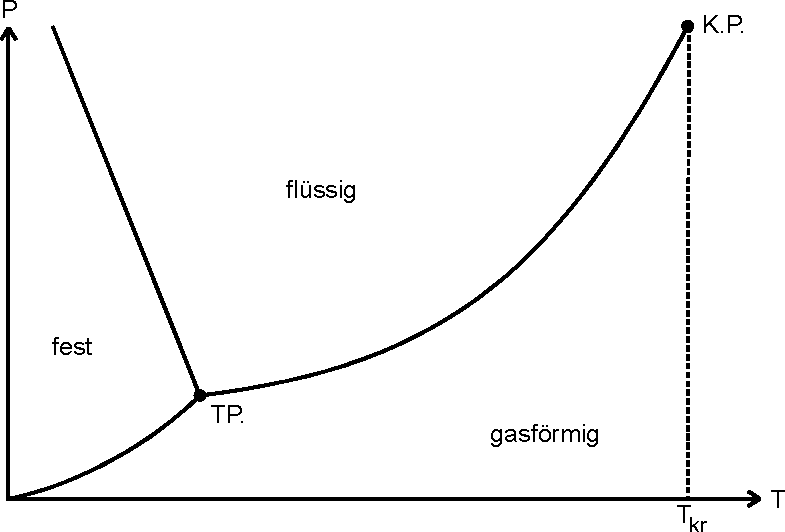
\includegraphics{Zustandsdiagramm.pdf}
    \caption{Qualitative Darstellung des Zustandsdiagramms von Wasser\cite{ap06}.}
    \label{fig:zustandsdiagramm}
\end{figure}

Das Wasser also für jeden Bezirk ohne Phasenübergang jeden Druck $p$ und jede Temperatur $T$ annehmen, die in diesem Bereich liegt.
In unmittelbarer Nähe zu einer der drei eingezeichneten Kurven existieren zwei Phasen nebeneinander, $p$ und $T$ sind nicht länger frei wählbar, die Anzahl der Freiheitsgrade des Systems reduziert sich von zwei auf einen Freiheitsgrad.
So ist der Druck bei gegebener Temperatur durch die jeweilige Kurve festgelegt. \\

Die beiden in \autoref{fig:zustandsdiagramm} hervorgehobenen Punkte T.P. und K.P. beschreiben den \textit{Tripelpunkt} bzw. den \textit{kritischen Punkt}.
Der Tripelpunkt beschreibt dabei den Punkt, bei dem alle drei Phasen des Wassers im thermodynamischen Gleichgewicht stehen, im kritischen Punkt besteht kein Unterschied mehr zwischen flüssiger und gasförmiger Phase. \\

Im Folgenden wird speziell die Dampfdruckkurve betrachtet.
Der Verlauf der Dampfdruckkurve wird insbesondere durch die temperaturabhängige Verdampfungswärme $L$ beeinflusst.
Sie beschreibt die Energie, die zur Umwandlung von einem Mol einer Flüssigkeit in Gas derselben Temperatur nötig ist.
Der Phasenübergang von flüssig nach gasförmig lässt sich an einer Flüssigkeit in einem evakuierten Gefäß veranschaulichen.
So lässt sich beobachten, dass ein Teil der Flüssigkeit in die Gasphase übergeht.
Dabei verlassen die Moleküle der gemäß der Maxwellschen Geschwindigkeitsverteilung höchsten kinetischen Energie die Flüssigkeit, dabei wird der Flüssigkeit Energie entzogen.
Durch Stöße mit den Gefäßwänden und der Flüssigkeitoberfläche entsteht ein vom Nulldruck des evakuierten Gefäßes abweichender Druck, die auf die Flüssigkeit treffenden Gasteilchen werden teilweise wieder eingefangen, sodass sich nach genügender Zeit ein Gleichgewicht
zwischen phasenübergehenden Teilchen einstellt.
Der dabei vorherrschende Druck wird als Sättigungsdampfdruck bezeichnet, der mit steigender Temperatur wächst und \textbf{nicht} vom Volumen des Gefäßes abhängt, also nicht der allgemeinen Gasgleichung folgt. 
Diese Verdampfungswärme verschwindet in der Nähe des kritischen Punktes, allerdings existiert auch ein Temperaturbereich, in dem $L$ nahezu konstant ist, in dem die Bestimmung der Dampfdruckkurve und der Verdampfungswärme stattfinden soll.

